% EXPERIMENTAL SETUP
% - Setup
%   \ac{DGI}
%   \ac{NS3}
%   Boost
% - Describe the setup -- Network layout, \ac{DGI} placement at nodes, Random seeds?
% - Describe the quantites we are looking at? What the graphs will mean. Establish the control-- normal operation.
% - Network behavior during the experiments.

\section{Experimental Setup}
\label{sect:experimentalsetup}

Experiments were run in a Network Simulator 3.23\cite{NS3} test environment.
The simulation time replaced the wall clock time in the \ac{DGI} for the purpose of triggering real-time events.
As a result, the computation time on the \ac{DGI}s for processing and preparing messages was neglected.
However, to compensate for the lack of processing time, the synchronization of the \ac{DGI}s was instead randomly distributed as a normal distribution.
This was done to introduce realism to ensure events did not occur simultaneously.
Additionally, the real-time schedules used by the \ac{DGI} were adjusted to remove the processing time that was neglected in the simulation.

The \ac{DGI}s were placed into a partitioned environment.
The test included 30 nodes.
Each of the nodes ran one \ac{DGI} process.
Two sets of 15 \ac{DGI} were each connect to a switch and each switch was in turn connected to the router.
This network is pictured in Figure \ref{fig:network-layout}.
Node identifiers were randomly assigned to nodes in the simulation and used as the process identifier for the \ac{DGI}.

The links between the router and the switches had a \ac{RED} enabled queue placed on both network interfaces.
The \ac{RED} parameters for all queues were set identically.
A summary of \ac{RED} parameters are listed in Table \ref{tab:red-parameters}.
All links in the simulation were 100Mbps links with a 0.5ms delay.
RED was used in packet count mode to determine congestion.
ARP tables were populated before the simulation began.

\ac{RED} parameters were selected using Equation \ref{eq:prob-est} and \cite{JOURNAL}.
The relationship between the background traffic and the average queue size was estimated through runs of the \ac{NS3} simulation.
Figure \ref{fig:plotm} demonstrates the observed relationship between the total background traffic and the maximum average queue size for that level of traffic.
Additionally, the $DequeueRate$ was collected from a run of the simulation without traffic, and was found to be $713.08$ packets/second.
Therefore, from Equation \ref{eq:prob-est}, assuming $init_q=0, resp=225, init_m=225$ and $\Delta t=1$, the maximum traffic rate with no omissions is $263.0$ packets/second.
The number of packets for the $resp$ and $init_m$ were selected from the worst case of the algorithm in \cite{JOURNAL}.
Based on the traffic parameters in Table \ref{tab:red-parameters}, $263.0$ packets/second corresponds to 1.077 Mbps of traffic generated at one switch and 2.1545 Mbps traffic overall.
From the polynomial estimate in Figure \ref{fig:plotm}, the maximum average queue size for that level of traffic is $94.715$, estimated as $90$ for the \ac{RED} Min Threshold in Table \ref{tab:red-parameters}.
RED Max Threshold is computed using a similar technique, but using the message complexity for the Load Balancing algorithm, since it maintains its complexity during Soft ECN mode.

\begin{figure}
\centering
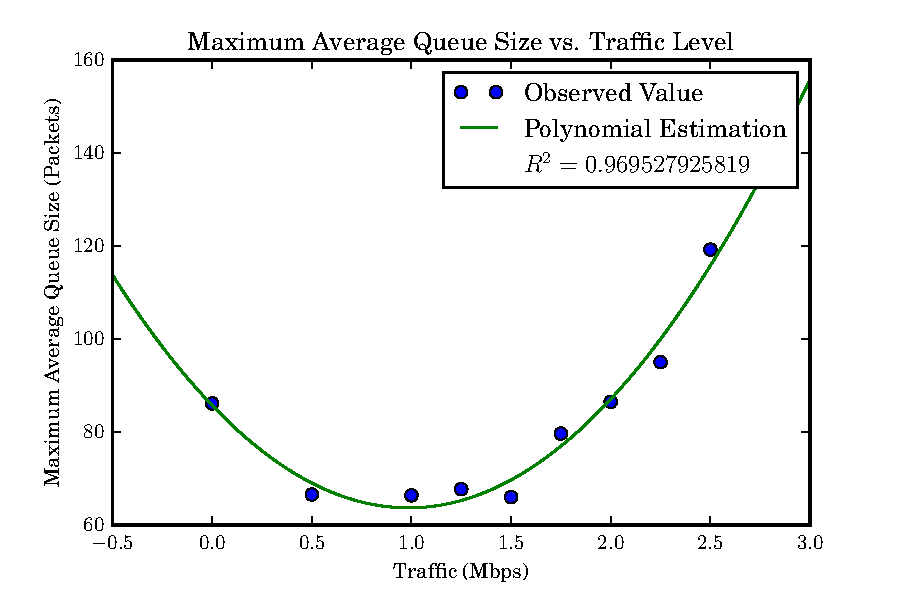
\includegraphics[width=0.65\linewidth]{m-max-average-queue.pdf}
\caption{Plot of the maximum observed average queue size as a function of the overall background traffic. The polynomial estimate is $y=22.70x^2-44.74x+85.72$}
\label{fig:plotm}
\end{figure}

\begin{table}
\begin{center}
\begin{tabular}{ | l | l | } \hline
Parameter & Value         \\ \hline
RED Queueing Mode & Packet\\ \hline 
RED Gentle Mode & True    \\ \hline
RED $Q_{w}$ & 0.002       \\ \hline
RED Wait Mode & True      \\ \hline
RED Min Threshold & 90    \\ \hline
RED Max Threshold & 130   \\ \hline
Maximum Queue Size & 1000 \\ \hline
RED Link Speed & 100 Mbps \\ \hline
RED Link Delay & 0.5 ms   \\ \hline
Clock Distribution $\sigma$ & 0.005 \\ \hline
Traffic Packet Size & 512 Bytes \\ \hline
\end{tabular}
\end{center}
\caption{Summary of \ac{RED} parameters. Unspecified values default to the \ac{NS3} implementation default value}
\label{tab:red-parameters}
\end{table}

To introduce traffic, processes attached to each of the switches attempted to send a high volume of messages to each other across the router.
The number of packets sent per second was a function of the data rate and the size of the packets sent.
In each simulation, half of the traffic originated from each switch.
Due to the bottleneck due to the properties of the network links, the greatest queueing effect occurred at the switches.
